\chapter{NVidia GPU指令集架构-整数运算}

\begin{center}\small 作者：reed（知乎 @reed-84-49，专栏「CUDA高性能编程」）\quad 原文：\url{https://zhuanlan.zhihu.com/p/700921948}\end{center}

前文我们介绍了NVidia GPU CUDA Core上的浮点运算指令(\url{https://zhuanlan.zhihu.com/p/695667044})，CUDA Core除了提供浮点能力外还提供了整数运算能力，整数运算能力在整个计算体系中扮演着至关重要的作用：如数据处理方面的统计、排序、计数、地址计算、索引；算法实现中的加密计算和验证。在大语言模型背景下，低比特的数据量化表示（如4bit量化）也是在对整数的进一步延伸，了解整数的表示以及其之上的运算是我们进行设计和优化的基础。本文将介绍NVidia GPU指令集架构中的整数运算指令。文章结构方面，首先介绍常用的整数类型和NVidia GPU的支持情况，然后介绍有符号整数的补码表示及其衍生的算术位移和逻辑位移的概念，然后文章具体介绍了NVidia GPU的整数相关的指令，最后对文章进行了总结。

\section{常用整数类型及其表示}

在计算机编程中，常用的整数数据类型有以下几种：

\lstinline|int8_t|、\lstinline|int16_t|、\lstinline|int32_t|、\lstinline|int64_t|、\lstinline|uint8_t|、\lstinline|uint16_t|、\lstinline|uint32_t|、\lstinline|uint64_t|，他们的占用的字体节数和数据范围如下表：

\begin{table}[htbp]\centering
\begin{tabular}{lllll}
\toprule
符号 & 类型 & 字节数 & 最大值 & 最小值 \\
\midrule
有符号 & \texttt{int8\_t} & 1 & -128 & 127 \\
有符号 & \texttt{int16\_t} & 2 & -32768 & 32767 \\
有符号 & \texttt{int32\_t} & 4 & -2147483648 & 2147483647 \\
有符号 & \texttt{int64\_t} & 8 & -9223372036854775808 & 9223372036854775807 \\
无符号 & \texttt{uint8\_t} & 1 & 0 & 255 \\
无符号 & \texttt{uint16\_t} & 2 & 0 & 65535 \\
无符号 & \texttt{uint32\_t} & 4 & 0 & 4294967295 \\
无符号 & \texttt{uint64\_t} & 8 & 0 & 18446744073709551615 \\
\bottomrule
\end{tabular}
\end{table}

\section{NVidia GPU对不同整数类型的支持}

NVidia GPU针对不同的计算精度需求提供了不同的整数精度和类型支持，具体地，在CUDA编程方面，它支持以上整数类型（\lstinline|int8_t|、\lstinline|int16_t|、\lstinline|int32_t|、\lstinline|int64_t|、\lstinline|uint8_t|、\lstinline|uint16_t|、\lstinline|uint32_t|、\lstinline|uint64_t|）的计算，在指令层面，由于NVidia GPU的寄存器为32bit，以加法为例对于小于等于32bit的计算，都使用同样的指令实现（IADD3指令），对于大于32bit的加法，则通过两条指令实现，分别计算低32bit加法结果和高32bit的加法结果，同时在计算低32bit的结果时，使用Predication寄存器(\url{https://zhuanlan.zhihu.com/p/688616037})保存其进位情况，在计算高32bit时同时附带上低32bit的进位结果。

\begin{figure}[htbp]\centering
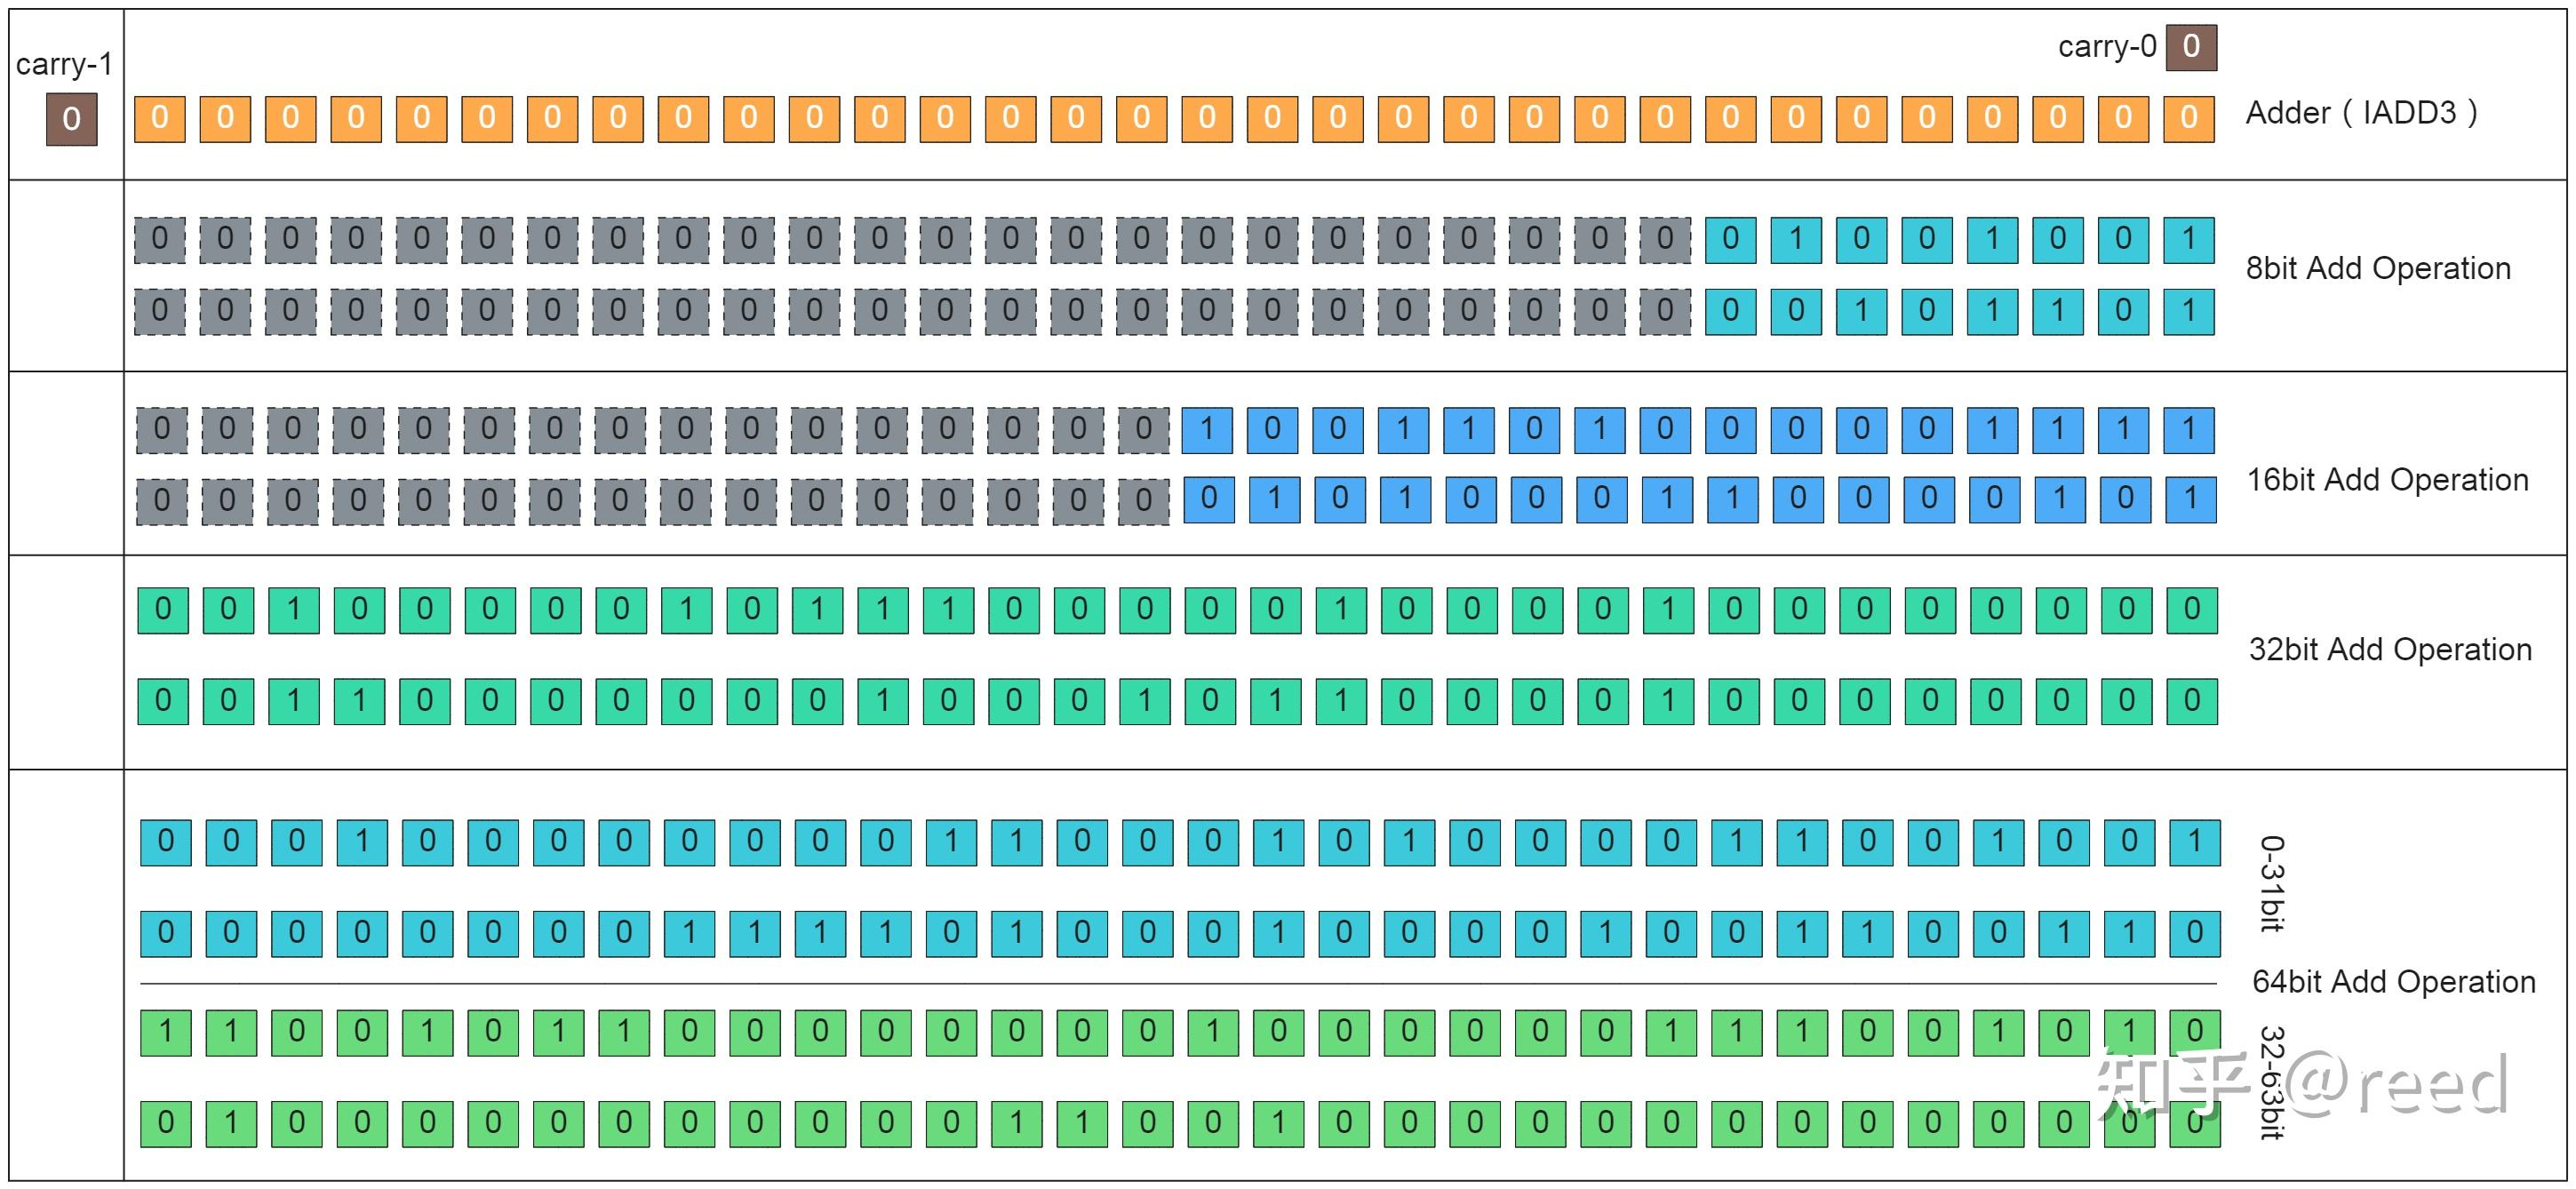
\includegraphics[width=0.9\textwidth]{figures/reed-isa-05-integer/fig-01.jpg}
\caption{Figure 1. 单一加法器支持不同精度的整数加法}
\end{figure}

如图1所示，GPU编程虽然语言层面支持不同的整数数据类型和精度，但硬件和指令集层面这些不同的类型加法都使用同一个加法器（如图1中的Adder），其为一个32bit的整数加法器其通过carry-0可以指定低位的进位情况同时通过carry-1表示加法的向上进位情况。对于8bit、16bit、32bit的加法，carry-0默认为0，8bit、16bit的数据在寄存器都被扩展为32bit，直接采用32bit的加法器进行计算，在存储结果时对结果进行截断即可（只保留低8bit、16bit）。对于64bit数据的加法，需要两阶段完成（编译器生成两条32bit加法指令），第一阶段计算低32bit的加法，和前面的计算过程类似，只需要carry-0设置为0进行计算，同时在计算过程中将carry-1保存在Predication寄存器中，第二阶段计算高32bit（即32-63bit），同时将第一阶段的carry-1设置为第二阶段的carry-0以确保进位被正确传递。

由于指令集方面只有32bit的计算指令，所以在GPU程序中采用低bit的整数计算并没有计算性能优势，反而低bit会引入截断指令，继而降低程序效率。对于大语言模型而言低bit量化可以减少内存使用量和数据IO开销，更多的是利用其存储空间优势，而非计算优势。

\section{有符号整数的补码表示和算术位移}

在计算机中为了简化了计算机内部的运算过程，统一加法和减法的处理，统一有符号和无符号运算，提高计算效率，在表示有符号数据时采用了补码的形式。计算机体系中数据都是通过多bit的0、1来表示，GPU也不例外。为了更好的表达有符号数据，可以在加法的基础上引申出负数的表示。如一个有符号的8bit的整数123，则其用原码表示为0x11110011，如图2所示，我们在加法意义上可以定义-123，使得它和123加起来后可以得到0（有符号8bit表示为0x00000000），那么如何定义-123可以满足这种加法逻辑呢，那就是先让123 + ? = 0x11111111，然后两边同时加1即可以在向上溢出的意义下满足全0。为了能得到全1我们可以针对123的二进制表示每个bit取反，然后把后面的+1也作用在-123的二进制表示上即可，这也就是教科书上的"取反加一"。这种取反加一的表示码称为补码（Two's Complement），即能够补（相加）为0的表示码，这样符号位也可参与运算，如此便形成了高位第一位（Most Significant Bit）表示符号位0表示正数，1表示负数。

\begin{figure}[htbp]\centering
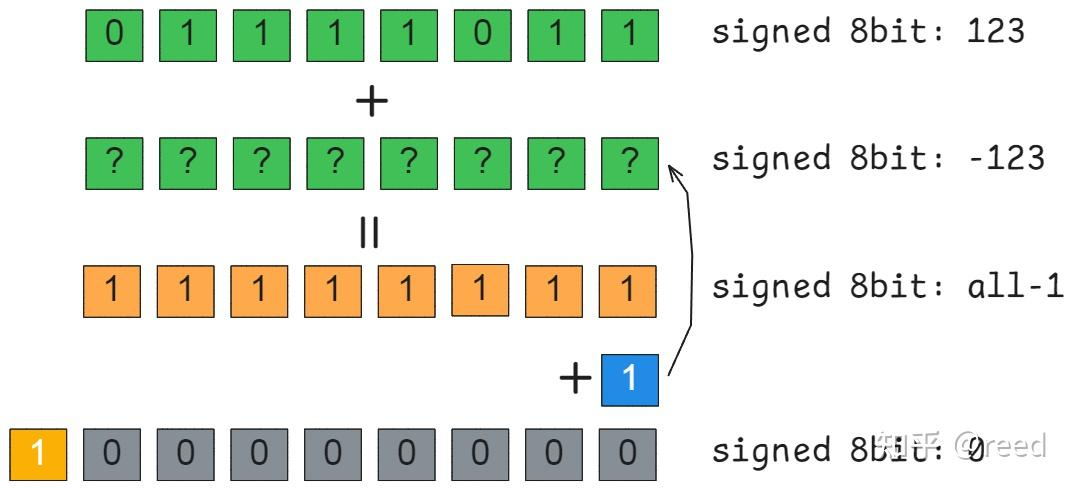
\includegraphics[width=0.9\textwidth]{figures/reed-isa-05-integer/fig-02.jpg}
\caption{Figure 2. 有符号数的补码表示}
\end{figure}

由于MSB表示符号，在进行比特级左右移时（Left or Right Shift），是否保留符号位产生了逻辑位移（Logical Shift）和算术位移（Arithmetic Shift）：

逻辑位移不考虑数的符号位，只是简单地将每一位向左或向右移动指定的位数，移出边界外的位将被舍弃，新的位置上会填充0。

\begin{itemize}
\item 逻辑左移：所有位向左移动，右边空出的位用0填充。
\item 逻辑右移：所有位向右移动，左边空出的位用0填充。
\end{itemize}

逻辑位移通常用于无符号数的运算，比如乘以2的幂次方（左移）或除以2的幂次方（右移）。

算术位移则考虑数的符号位，主要用于保持数值的符号不变。

\begin{itemize}
\item 算术左移：与逻辑左移相同，所有位向左移动，右边空出的位用0填充。
\item 算术右移：所有位向右移动，但左边空出的位会根据原数的符号位填充，若原数为正，则填充0；若原数为负，则填充1。
\end{itemize}

算术位移通常用于有符号数的运算，尤其是除法运算时，它能够保持数值的正负号不变。

在NVidia GPU指令方面，逻辑位移和算术位移统一为SHF指令，通过有符号和无符号类型作为Modifier来实现对符号位的保留与否。针对大模型中的低bit量化，通常采用的是算术位移，同时附加上其他的逻辑操作实现低bit的数据合并和表示。

\section{NVidia GPU整数指令集}

NVidia GPU指令集架构提供了针对整数的各种计算和操作，该章节分类介绍各个计算相应的指令。值得注意的是不同的GPU架构整数计算和浮点计算的吞吐有很大差别(\url{https://docs.nvidia.com/cuda/cuda-c-programming-guide/index.html#arithmetic-instructions})，选择合适的计算类型能有效的提升程序性能，切记不要简单的以为整数效率比浮点高。

\subsection{整数加法}

整数加法通过\lstinline|IADD3|（Integer ADD 3 operand）实现（\lstinline|d = a + b + c|），一般形式如下, 其中8bit、16bit、32bit的加法共用如下形式1，针对64bit的加法，示例中P0为输出寄存器，类型为Predication Register，其功能如图1中的carry-0，用以输出低32bit计算时的进位情况，然后将这个进位带给高32bit的计算\lstinline|IADD3.X|，通过这两条指令实现64bit的加法。整数减法通过随路取符号实现，同时将b c都设置为0， 则实现取相反数的能力（negate）即 \lstinline|d = -a|。

\begin{lstlisting}
// 8bit, 16bit, 32bit
IADD3 R7, R0, R7, RZ ; // R7 = R0 + R7 + RZ

// substraction
IADD3 R7, R0, -R7, RZ ;

// 64bit R6-7 = R4-5 + R6-7
IADD3 R6, P0, R4, R6, RZ ;  // (R6, P0) = R4 + R6 + R0; P0 indicate carry
IADD3.X R7, R5, R7, RZ, P0, !PT ; // R7 = R5 + R7 + RZ + P0;
\end{lstlisting}

\subsection{整数乘法}

指令集没有提供独立的整数乘法，而是以乘加合并的形式提供（Integer Multiply ADd），提供形如 \lstinline|d = a x b + c| 的整数计算能力，除了标准能力外，该指令还以Modifier的形式提供了，只算高32bit的HI；通过a、b、c给特定值实现\lstinline|MOV(a = 0, b = 0)|，\lstinline|ADD|语义\lstinline|(b = 1)|，\lstinline|SHL|语义（\lstinline|b = 2,4,..|）,以及64bit的支持WIDE，常见的带Modifier指令如下, 对于c可以随路取负实现 \lstinline|d = a x b - c| 的计算语义：

\begin{lstlisting}
IMAD
IMAD.HI
IMAD.HI.U32
IMAD.IADD
IMAD.IADD.U32
IMAD.MOV
IMAD.MOV.U32
IMAD.SHL
IMAD.SHL.U32
IMAD.U32
IMAD.U32.X
IMAD.WIDE
IMAD.WIDE.U32
IMAD.WIDE.U32.X
IMAD.X
\end{lstlisting}

\subsection{整数位移}

位移（SHFit）通过Modifier指定移动方向向左（Left）或者向右（Right），同时通过U32、U64等指定类型和或逻辑位移，通过S32、S64指定类型和或算术位移。

\begin{lstlisting}
SHF.L.U32
SHF.L.U32.HI
SHF.L.U64.HI
SHF.L.W.U32
SHF.R.S32.HI
SHF.R.S64
SHF.R.U32.HI
SHF.R.U64
\end{lstlisting}

\subsection{整数除法和取余}

NVidia GPU指令集架构中并没有提供独立的整数除法指令，而是先将整数转换为浮点数，通过SFU（Special Function Unit提供的倒数指令，参看浮点计算中的除法(\url{https://zhuanlan.zhihu.com/p/695667044})）完成除法计算，然后再转换为整数进行结果修正。对于除数为编译时常量的，编译器会使用数学变换将该除法变换成更简单的位移和乘法指令(\url{https://gmplib.org/~tege/divcnst-pldi94.pdf})，cutlass中也有类似实现(\url{https://github.com/NVIDIA/cutlass/blob/main/include/cutlass/fast_math.h#L364})。

\subsection{整数转浮点数}

对于整数和浮点数类型的转换（Integer 2：to Float），默认为int32转换为float32，指令集也提供了相应的功能，通过Modifier提供更细节的修饰，涉及整数到float16（F16）、float64（F64）类型，同时源操作数也区分是有符号和无符号，和低精度(S8、S16、S64、U16、U32、U64)，以及Round Positive（RP）:

\begin{lstlisting}
I2F
I2F.F16
I2F.F64
I2F.F64.S64
I2F.F64.U32
I2F.F64.U64
I2F.RP
I2F.S16
I2F.S64
I2F.S8
I2F.U16
I2F.U32
I2F.U32.RP
I2F.U64
I2F.U64.RP
\end{lstlisting}

\subsection{整数转Packed整数}

指令集除了提供整数和浮点数的转换，还提供了整数和packed整数的转换（Integer 2：to Integer Packed ）来避免使用更复杂的逻辑和位移实现，如下

\begin{lstlisting}
I2IP.S8.S32.SAT
\end{lstlisting}

\subsection{整数绝对值}

原生提供了绝对值计算指令IADD（Integer ABSolute）

\begin{lstlisting}
IABS
\end{lstlisting}

\subsection{整数点积}

针对低精度整数的点积运算（Integer Dot Product），对于深度学习场景，针对特别小的channel，利用该指令可以实现较好的效果：

\begin{lstlisting}
IDP.2A.LO.U16.U8
IDP.4A.S8.S8
\end{lstlisting}

\subsection{整数最大最小}

指令集提供整数两个数据比较大小的操作（Integer MiNimum and MaXimum），同时选取出其中的大数据或小数，避免使用条件分支实现，同时提供了针对数据类型Unsigned Integer的Modifier，对于32bit及以下数据都可以使用该指令实现，对于64bit数据使用\lstinline|ISETP|实现：

\begin{lstlisting}
IMNMX R7, R0, R7, !PT ; // when PT return R7 = min(R0, R7), when !PT R7 = max(R0, R7)
IMNMX.U32
\end{lstlisting}

\subsection{整数比较产生条件}

对于更复杂的比较和逻辑（Integer SET Predicate），常见的整数相关的条件如下，组合它们可以得到更复杂的控制逻辑：

\begin{lstlisting}
ISETP.EQ.AND      ISETP.EQ.U32.OR  ISETP.GE.OR.EX       ISETP.GT.AND.EX      ISETP.GT.U32.OR   ISETP.LT.AND      ISETP.LT.U32.AND.EX  ISETP.NE.OR.EX
ISETP.EQ.AND.EX   ISETP.EQ.XOR     ISETP.GE.U32.AND     ISETP.GT.OR          ISETP.LE.AND      ISETP.LT.AND.EX   ISETP.LT.U32.OR      ISETP.NE.U32.AND
ISETP.EQ.OR       ISETP.GE.AND     ISETP.GE.U32.AND.EX  ISETP.GT.OR.EX       ISETP.LE.OR       ISETP.LT.OR       ISETP.NE.AND         ISETP.NE.U32.AND.EX
ISETP.EQ.OR.EX    ISETP.GE.AND.EX  ISETP.GE.U32.OR      ISETP.GT.U32.AND     ISETP.LE.U32.AND  ISETP.LT.U32.AND  ISETP.NE.OR
ISETP.EQ.U32.AND  ISETP.GE.OR      ISETP.GT.AND         ISETP.GT.U32.AND.EX  ISETP.LE.U32.OR   ISETP.LT.OR.EX    ISETP.NE.OR
\end{lstlisting}

\subsection{Tensor Core整数指令}

另外NVidia GPU通过Tensor Core提供了算力更高的整数类型矩阵乘法指令，我们会在后面章节更详细的介绍：

\begin{lstlisting}
IMMA.16816.S8.S8
IMMA.16832.S8.S8.SAT
IMMA.8816.S8.S8.SAT
\end{lstlisting}

\section{总结}

本文介绍了编程中常用的整数类型和NVidia GPU的统一加法器逻辑对它们的支持情况，同时介绍了有符号数的补码表示以及其衍生出的算术位移和逻辑位移的区别，最后文章详细介绍了NVidia GPU针对整数运算的各种指令，了解整数的表示和计算逻辑以及底层指令能帮助我们选择合适的计算精度，其对更高阶的优化有重要的指导意义。

\section{参考}

\url{https://gmplib.org/~tege/divcnst-pldi94.pdf}

\url{https://github.com/NVIDIA/cutlass/blob/main/include/cutlass/fast_math.h#L364}

\url{https://docs.nvidia.com/cuda/cuda-c-programming-guide/index.html#arithmetic-instructions}

reed：NVidia GPU指令集架构-寄存器(\url{https://zhuanlan.zhihu.com/p/688616037})

reed：NVidia GPU指令集架构-浮点运算(\url{https://zhuanlan.zhihu.com/p/695667044})
